\chapter{System Architecture}
\label{chap:architecture}

The previous chapters introduced the core building blocks: the \texttt{UiService} for managing UI state (Chapter~\ref{chap:ui-service}), the Petri net elements as data objects (Chapter~\ref{chap:petri-net-elements}), and the \texttt{DataService} as the central data store (Chapter~\ref{chap:data-service}). This chapter provides a high-level overview of how these components fit together within the overall system architecture.

\section{System Overview}
\label{sec:system-overview}

The L3S-Offshore-2 system follows a client-server architecture with clear separation between the visualization frontend and the simulation backend.

\begin{figure}[htb]
    \centering
    \begin{tikzpicture}[
        node distance=1.5cm,
        box/.style={rectangle, draw, minimum width=3.5cm, minimum height=1cm, align=center, font=\small},
        arrow/.style={->, thick},
    ]
        % Frontend
        \node[box, fill=green!15] (fe) {Angular Frontend\\(Browser)};
        
        % Backend
        \node[box, fill=blue!15, right=4cm of fe] (be) {Flask Backend\\(Python)};
        
        % Database/Storage
        \node[box, fill=orange!15, below=of be] (db) {Example Models\\(File Storage)};
        
        % Arrows
        \draw[arrow] ([yshift=3pt]fe.east) -- node[above, font=\scriptsize] {HTTP POST (PNML)} ([yshift=3pt]be.west);
        \draw[arrow] ([yshift=-3pt]be.west) -- node[below, font=\scriptsize] {JSON (Results)} ([yshift=-3pt]fe.east);
        \draw[arrow] (be) -- (db);
        
    \end{tikzpicture}
    \caption{High-level system architecture showing frontend-backend interaction}
    \label{fig:system-architecture}
\end{figure}

\subsection{Frontend (Angular)}

The frontend is a single-page application (SPA) responsible for:
\begin{itemize}
    \item Rendering Petri nets as interactive SVG graphics
    \item Handling user interactions (editing, navigation, simulation control)
    \item Managing application state across different tabs
    \item Communicating with the backend via REST API
\end{itemize}

\subsection{Backend (Flask)}

The Python backend provides:
\begin{itemize}
    \item PNML parsing and validation
    \item Petri net simulation using the \texttt{gspn4py} library
    \item Offshore scheduling algorithms
    \item Example model storage and retrieval
\end{itemize}

\section{Frontend Component Hierarchy}
\label{sec:component-hierarchy}

The Angular application is organized into a hierarchical component structure that reflects the UI layout.

\subsection{Root Components}

\begin{description}
    \item[AppComponent] The root component that bootstraps the application and contains the main layout
    \item[HeaderComponent] Displays the project banner with L3S branding
    \item[FooterComponent] Shows institutional logos with links to L3S and LUH homepages
\end{description}

\subsection{Tab Components}

The main content area uses Angular Material's tab group:

\begin{description}
    \item[ButtonBarComponent] The central coordinator that manages tab switching and toolbar rendering for each tab (Build, Code, Simulation, Analyze, Save, Offshore)
    \item[PetriNetComponent] Renders the interactive SVG visualization of the Petri net
    \item[CodeEditorComponent] Provides a text editor for direct PNML manipulation
    \item[ParameterTableComponent] Displays and edits simulation parameters
    \item[OffshoreViewComponent] Specialized view for offshore scheduling parameters
\end{description}

\subsection{Dialog Components}

Modal dialogs for user feedback and interaction:
\begin{description}
    \item[DataPersistenceInfoDialogComponent] Warns users about data loss on page reload
    \item[ErrorPopupComponent] Displays error messages from backend or parsing failures
    \item[HelpPopupComponent] Provides contextual help
    \item[TransitionFiringInfoPopupComponent] Shows firing statistics for transitions
\end{description}

\section{Service Layer}
\label{sec:service-layer}

Services are singleton classes that provide shared functionality and state management. The most important services are covered in dedicated chapters.

\subsection{Core Services}

\begin{description}
    \item[DataService] Central state container for the Petri net model. Manages places, transitions, arcs, and the current marking. Emits change events via RxJS observables. \textit{See Chapter~\ref{chap:data-service} for details.}
    
    \item[UiService] Manages UI state including the current tab, simulation mode (automatic/manual), selected elements, and zoom level. \textit{See Chapter~\ref{chap:ui-service} for details.}
    
    \item[ZoomService] Handles viewport transformations (pan, zoom) with ResizeObserver integration for responsive behavior. \textit{See Section~\ref{sec:zoom-pan-system} for details.}
    
    \item[ParserService] Converts between PNML XML, internal data structures, and the JSON representation used by the backend. \textit{See Chapter~\ref{chap:data-io} for details.}
\end{description}

\subsection{Simulation Services}

\begin{description}
    \item[SimulationService] Communicates with the backend's simulation endpoints. Manages firing sequences and multi-run results.
    
    \item[TokenGameService] Implements the manual simulation mode where users can step through the firing sequence or click on enabled transitions.
    
    \item[PlanningService] Handles the offshore scheduling API calls and parameter management. \textit{See Chapter~\ref{chap:planning-service} for details.}
\end{description}

\subsection{Utility Services}

\begin{description}
    \item[ExportImageService] Exports the current view as PNG
    \item[ExportSvgService] Exports the Petri net as SVG
    \item[ExportJsonDataService] Exports the internal representation as JSON. \textit{See Chapter~\ref{chap:data-io} for details.}
    \item[LayoutSugiyamaService] Implements the Sugiyama algorithm for automatic layout. \textit{See Chapter~\ref{chap:layout-algorithms} for details.}
\end{description}

\section{Data Flow}
\label{sec:data-flow}

\begin{figure}[htb]
    \centering
    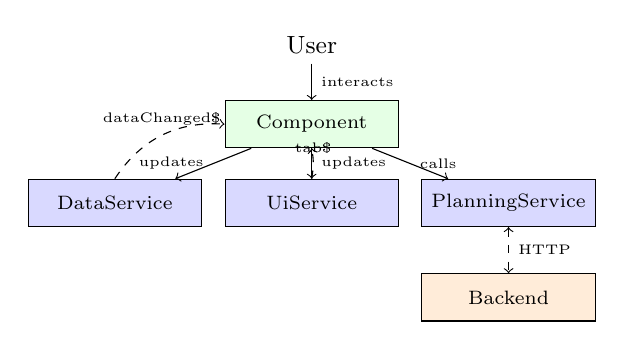
\begin{tikzpicture}[
        node distance=0.8cm,
        component/.style={rectangle, draw, fill=green!10, minimum width=2.2cm, minimum height=0.6cm, font=\scriptsize},
        service/.style={rectangle, draw, fill=blue!15, minimum width=2.2cm, minimum height=0.6cm, font=\scriptsize},
    ]
        % User
        \node (user) at (0, 2) {\small User};
        
        % Components
        \node[component] (comp) at (0, 1) {Component};
        
        % Services
        \node[service] (data) at (-2.5, 0) {DataService};
        \node[service] (ui) at (0, 0) {UiService};
        \node[service] (plan) at (2.5, 0) {PlanningService};
        
        % Backend
        \node[component, fill=orange!15] (back) at (2.5, -1.2) {Backend};
        
        % Arrows
        \draw[->] (user) -- node[right, font=\tiny] {interacts} (comp);
        \draw[->] (comp) -- node[left, font=\tiny] {updates} (data);
        \draw[->] (comp) -- node[right, font=\tiny] {updates} (ui);
        \draw[->] (comp) -- node[right, font=\tiny] {calls} (plan);
        \draw[<->, dashed] (plan) -- node[right, font=\tiny] {HTTP} (back);
        \draw[->, dashed] (data.north) to[bend left=30] node[above, font=\tiny] {dataChanged\$} (comp.west);
        \draw[->, dashed] (ui.north) to[bend right=10] node[above, font=\tiny] {tab\$} (comp.south);
        
    \end{tikzpicture}
    \caption{Data flow between components and services}
    \label{fig:data-flow}
\end{figure}

The application follows a unidirectional data flow pattern:

\begin{enumerate}
    \item \textbf{User Input:} User interacts with UI (clicks, drags, edits)
    \item \textbf{Component Handler:} Component method processes the event
    \item \textbf{Service Update:} Component calls service method to update state
    \item \textbf{Observable Emission:} Service emits new state via RxJS Subject
    \item \textbf{Subscriber Notification:} All subscribed components receive update
    \item \textbf{View Re-render:} Angular change detection updates the DOM
\end{enumerate}

\section{Tab State Management}
\label{sec:tab-state-management}

A key architectural feature is the tab-aware state management that ensures UI consistency when switching between tabs.

\subsection{The Tab\$ Observable}

The \texttt{UiService} exposes a \texttt{tab\$} BehaviorSubject that emits the current tab name whenever the user navigates:

\begin{lstlisting}[language=TypeScript, caption={Tab state observable in UiService}]
private _tab$ = new BehaviorSubject<string>('build');

get tab$(): Observable<string> {
  return this._tab$.asObservable();
}

set tab(value: string) {
  console.log(`[UiService] Tab changed: ${this._tab$.value} -> ${value}`);
  this._tab$.next(value);
}
\end{lstlisting}

\subsection{Tab Guards in Components}

Components subscribe to \texttt{tab\$} and conditionally enable/disable features:

\begin{lstlisting}[language=TypeScript, caption={Tab-aware highlighting in PetriNetComponent}]
this.uiService.tab$.subscribe(tab => {
  if (tab !== 'simulation') {
    this.clearAllHighlights();
    this.stopAnimationTimer();
  } else {
    this.restoreSimulationState();
  }
});
\end{lstlisting}
